%===================================================================================
% Chapter: Propuesta para la Extracción de Entidades
%===================================================================================
\chapter{Propuesta para la Extracción de Entidades}\label{chapter:entities}
\addcontentsline{toc}{chapter}{Extracción de Entidades}
%===================================================================================

%===================================================================================

En este capítulo se hace una descripción de las técnicas empleadas para la resolución de la tarea de Extracción de Entidades, donde se describe como funciona el modelo de aprendizaje profundo propuesto, la construcci\'on de su entrada a partir de una oraci\'on, entre ellas la obtenci\'on de los \emph{embeddings contextuales} de las palabras de una oraci\'on hacienqdo uso de un modelo preentrenado de BERT. Finalmente se describe cada una de las componentes del modelo de aprendizaje profundo y su funcionamiento.


\section{Modelo de Aprendizaje Profundo}

El modelo propuesto es un BiLSTM-CRF apilado que tiene como entrada \emph{embeddings contextuales} pre-entrenados con BERT, \emph{postag embeddings} que son entrenados junto al modelo y \emph{character embeddings} que se entrenan junto al modelo a partir de una CNN. El modelo tiene como decodificador para la predicci\'on de las etiquetas correspondientes a cada token un CRF. El modelo pretende determinar cu\'ales son las entidades dentro de la oraci\'on y de esas entidades cu\'al es su clasificaci\'on como \emph{Concepto}, \emph{Acci\'on}, \emph{Predicado} y \emph{Referencia}.

\subsection{Entrada del Modelo}\label{sec:entrance}
Se recibe como entrada una oraci\'on en texto plano, la cual necesita preprocesamiento para construir la entrada apropiada del modelo. El primer paso es tokenizar las oraciones dado que todas las entradas del modelo esperan una secuencia de tokens. Para esto se utiliza la tokenizaci\'on a nivel de palabras.

Por cada token en el cual una oraci\'on fue dividida, la entrada respectiva a ese token consiste de una lista de tres vectores de rasgos.

\begin{description}
	\item[Vector de PoS-tag:] Es un vector \emph{one-hot} de codificaci\'on de la informaci\'on de \emph{Part of Speech} (PoS).
	\item[Codificaci\'on de los caracteres:] Es la concatenaci\'on de los vectores \emph{one-hot} de codificaci\'on de cada uno de los caracteres contenidos en la palabra. 
	\item[Embedding Contextual:] Es un vector de \emph{embedding} de la palabra conformado por la concatenaci\'on de los vectores que representan a dicha palabra en cada una de las capas de BERT.
	 
\end{description} 

Para extraer la informaci\'on de \emph{PoS-tag} se utiliza la librer\'ia de python \texttt{spacy}~\footnote{spacy.io}. 

Para la construcci\'on de los \emph{emmbeddings contextuales} correspondientes a cada token se utiliza un modelo preentrenado de \textbf{BERT}, siguiendo el siguiente procedimiento. Se toma la oraci\'on y se le agregan al inicio y al final las cadenas de texto \emph{"[CLS]"} y \emph{"[SEP]"} respectivamente. Luego esta nueva oraci\'on es tokenizada utilizando un algoritmo de tokenizaci\'on de subpalabras conocido como \emph{Word Piece}~\cite{schuster2012japanese}. El vocabulario de \emph{Word Piece} de BERT se computa aplicando el algoritmo de \emph{Word Piece tokenization} en cada secuencia de caracteres del corpus en el que se entren\'o BERT: \emph{Wikipedia and the Book Corpus}, lo cual resulta en 30 mil tokens de vocabulario. Como es l\'ogico, debido al tipo de tokenizaci\'on \emph{Word Piece}, se quisiera distinguir dentro del vocabulario a las palabras \emph{venoso} como una sola palabra y el sufijo \emph{venoso}, por lo que el sufijo se representa de la forma \emph{\#\#venoso} en el vocabulario.

%por el \emph{BertTokenizer} de la biblitoeca \textbf{pytorch-pretrained-bert}~\footnote{https://pypi.org/project/pytorch-pretrained-bert/} utilizando un algoritmo de tokenizaci\'on de subpalabras conocido como \emph{Word Piece}~\cite{schuster2012japanese}. 

%La tokenizaci\'on de \emph{Word Piece} es en esencia la idea de un algoritmo de compresi\'on, en este caso de representar palabras frecuentes con menos s\'imbolos y palabras menos frecuentes con m\'as s\'imbolos lo cual es de hecho la idea que hay detr\'as de varios esquemas de codificaci\'on como la codificaci\'on de \emph{Huffman}. \emph{Word Piece aplica el mismo principio} y t\'ecnicas a la tokenizaci\'on. \emph{Word Piece} es un algoritmo \emph{bottom- up} para la tokenizaci\'on de subpalabras que aprende un vocabulario de subpalabras de cierto tama\~no. La idea b\'asica es la siguiente:
%
%\begin{enumerate}
%	\item Comienza separando todas las palabras en caracteres unicode. Cada caracter unicode corresponde a un s\'imbolo en el vocabulario final. Se comienza con este vocabulario minimalista y luego se expande.
%	\item Mientras a\'un haya espacio en el vocabulario se hace lo siguiente:
%	\begin{enumerate}
%		\item Encontrar la pareja (\emph{bigram}) de s\'imbolos tal que al mezclarla incrementa the likelihood de un modelo de lenguaje unigram entrenado en los datos de entrenamiento. Este tipo de mezcla adem\'as de la frecuencia de la pareja de s\'imbolos, tiene en cuenta la frecuencia de los s\'imbolos del vocabulario inicial que los conforman. La log likelihood de una oraci\'on en una modelo de lenguaj unigram (asumiendo independencia entre las palabras) es la suma de las frecuencias de los s\'imbolos que los componen. Esto significa que mezclar dos s\'imbolos incrementa el total de la log likelihood por el log likelihood de los dos s\'imbolos mezclados y disminuir por los log likelihod de los dos s\'imbolos originales. Asumiendo que se mezclan \emph{x} y \emph{y}, el incremento en el log likelihood total ser\'ia de:
%		
%		\begin{equation}
%			\log p(x,y) - \log p(x) - \log p(y) = \log \frac{\log(p(x))}{\log(p(x))\log(p(y))}
%		\end{equation}
%		
%		\item Mezclar esos dos s\'imbolos para crear un nuevo s\'imbolo y a\~nadirlo al vocabulario. Esto incrementa el tama~no del vocabulario en 1.
%	\end{enumerate}
%	
%\end{enumerate} 

Posteriormente los tokens obtenidos tras tokenizar la oraci\'on utilizando el \emph{Word Piece tokenizer} son llevados a \'indices con respecto al vocabulario de BERT. Adem\'as se contruye la m\'ascara de atenci\'on poniendo a todos los tokens el valor de \textbf{1}, dado que no es necesario para nuestros objetivos hacer \emph{padding} de las oraciones. Luego la secuencia de \'indices de los tokens en el vocabulario de BERT y la m\'ascara de atenci\'on son pasadas como entrada del modelo pre-entrenado de BERT, obteniendo as\'i como salida la codificaci\'on de cada una de las capas de BERT para cada una de las palabras.

Luego el \emph{embedding contextual} de cada token se construye a partir de la concatenaci\'on de la codificaci\'on de dicho token en las \textbf{n} capas de BERT, o sea, si el token $t$, tiene codificaciones $l_1, l_2, ..., l_n$ en cada una de las capas de BERT respectivamente, entonces el \emph{embedding contextual} del token $t$ ser\'ia la concatenaci\'on de cada una de las codificaciones anteriores, resultando en el vector: $l_1l_2....l_n$.

Sin embargo, debido a la tokenizaci\'on del tipo \emph{Word Piece} realizada, hay palabras que quedan separadas en varios tokens, como por ejemplo \emph{[c\'an], [\#\#cer]}, donde la palabra \emph{c\'ancer} es una entidad y se clasificar\'ia como \emph{Concepto}, pero para que la arquitectura del modelo de aprendizaje profundo pueda etiquetar correctamente a la palabra c\'ancer, tendr\'ia que etiquetar dos tokens en vez de uno, por eso para la entrada del modelo de aprendizaje profundo para resolver la \emph{Subtarea A} se utiliza el tokenizer a nivel de palabras y no el tokenizer de BERT. Por lo que queda el problema de que al obtener, del modelo pre-entrenado de BERT, los \emph{embeddings contextuales} de cada uno de los tokens obtenidos de la \emph{Word Piece tokenization} es necesario computar cu\'al ser\'ia el \emph{embedding contextual} de los tokens obtenidos por la tokenizaci\'on a nivel de palabras. Luego para lograr este objetivo se dise\~na un algoritmo de \textbf{mapping}. 

El algoritmo de \emph{mapping} consiste b\'asicamente en la siguiente idea. Sea \emph{w} un token obtenido por la tokenizaci\'on por espacios y basada en reglas y los tokens $t_1, t_2, ..., t_k$ tokens obtenidos por el tokenizer de BERT tales que:

\begin{equation}
	w = \sum_{i = 1}^{k} t_i
\end{equation} 


y sean $e_1, e_2, ..., e_k$ los \emph{embeddings contextuales} obtenidos a partir de BERT para cada uno de los tokens $t_i$ ($1 \leq  i \leq k$), entonces sea $e_t$ el  \emph{embedding contextual} correspondiente al token $t$, el mismo se obtendr\'ia de la siguiente forma:

\begin{equation}
	e_t = mean(e_1, e_2, ... , e_k)
\end{equation}

Donde \emph{mean} es la funci\'on que devuelve la media de los vectores $e_1, e_2, ..., e_k$. De esat forma se obtiene un \emph{mapping} de los \emph{embeddings contextuales} de BERT para los \emph{word piece tokens} hacia los tokens obtenidos a por la tokenizaci\'on a nivel de palabras.

\subsection{Arquitectura del Modelo}

El modelo recibe una secuencia $S$ de tokens como entrada tal y como fue descrito en~\ref{sec:entrance}. La arquitectura se divide en tres niveles: (1) representaci\'on de los \emph{tokens}, (2) respresentaci\'on de la secuencia, y (3) predicci\'on de las etiquetas \emph{BMEWO-V} y la clasificaci\'on seg\'un las etiquetas \emph{Concept}, \emph{Action}, \emph{Reference}, \emph{Predicate} y \emph{None}, esta \'ultima en caso de no pertenecer a ninguna de las anteriores. La figura~\ref{fig:ArcModRec} y~\ref{fig:ArcModClass} resumen la arquitectura del modelo.


\begin{figure}[h!]
	\centering
	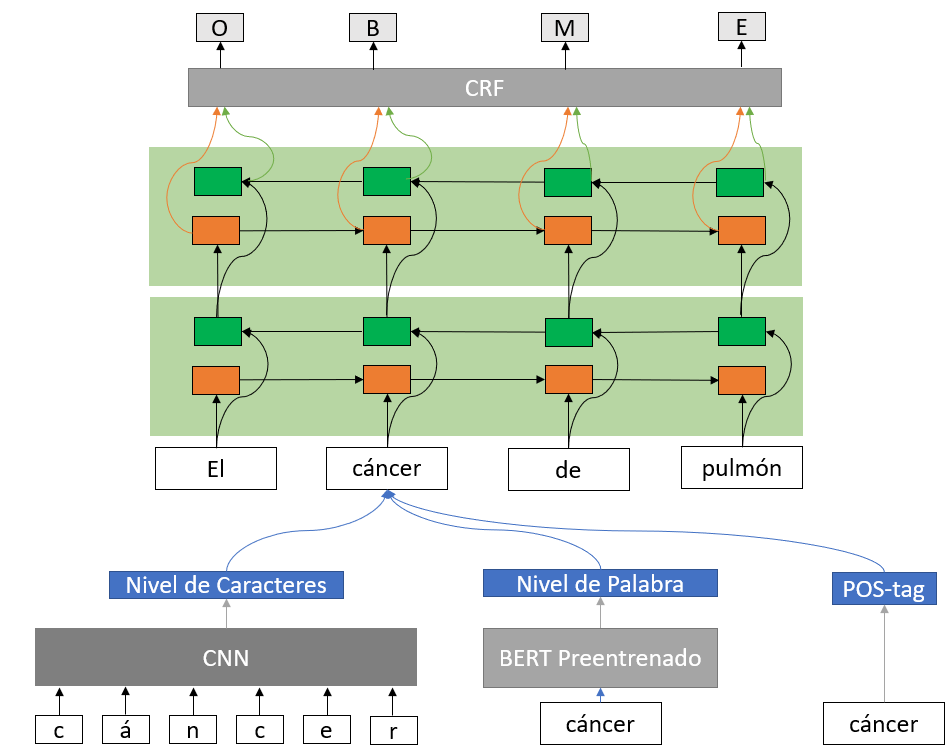
\includegraphics[width = 10cm]{Imagenes/EntitiesModelRec.png}
	\caption{Arquitectura del modelo de aprendizaje profundo para la extraccio\'on y clasificaci\'on de entidades con el CRF para la decodificaci\'on de las etiquetas \emph{BMEWO-V}.}\label{fig:ArcModRec}
\end{figure}

\begin{figure}[h!]
	\centering
	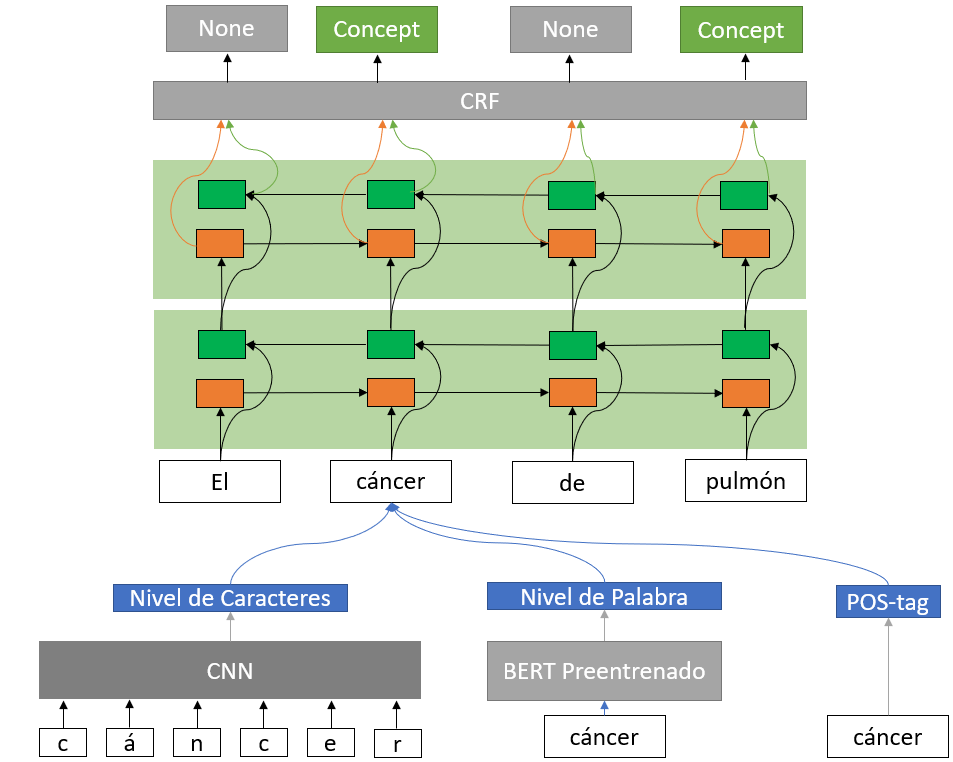
\includegraphics[width = 10cm]{Imagenes/EntitiesModelClas.png}
	\caption{Arquitectura del modelo de aprendizaje profundo para la extraccio\'on y clasificaci\'on de entidades con el CRF para la decodificaci\'on de las etiquetas de clasificaci\'on \emph{Concept}, \emph{Action}, \emph{Reference}, \emph{Predicate} y \emph{None},}\label{fig:ArcModClass}
\end{figure}

En un primer nivel, el modelo se encarga de obtener la representaci\'on de cada token en la secuencia de entrada, para ello existe una capa intermedia que trabaja en funci\'on de transformar la caracter\'istica \emph{Char Indexes} en vectores, que junto al de \emph{PosTag} y el \emph{embedding contextual} forman la representaci\'on final del token. Una capa CNN convierte los \emph{Char Indexes} en un vector de \emph{embedding} que atrapa el significado sem\'antico del token a nivel de caracteres. Esto se incluye para que el modelo se auxilie de caracter\'isticas morfol\'ogicas de la palabra (como prefijos y sufijos) en caso de que el token no forme parte del vocabulario del modelo de BERT preentrenado. El vector obtenido a partir de la CNN concatenado con el vector de \emph{embedding contextual} y el de \emph{PosTag} forman la representaci\'on del token.

En un segundo nivel, el modelo procesa la secuencia de tokens para obtener representaciones a nivel de oraci\'on. Una capa BiLSTM recorre la secuencia de tokens en ambos sentidos para construir dos secuencias de vectores. Los vectores en posiciones complementarias de las dos secuencias son concatenados, obteni\'endose as\'i nuevamente una secuencia $P$ que asocia un vector dependiente del contexto, que captura informaci\'on de la oraci\'on completa, a cada token de la oraci\'on. Esta secuencia busca atrapar las dependencias semánticas entre los tokens de la oración.
Luego una segunda BiLSTM apilada, que se utiliza tradicionalmente para a\~nadir m\'as poder representacional, recorre la secuencia devuelta por la primera BiLSTM en ambos sentidos, para tambi\'en construir dos secuencias de vectores que son concatenadas, produciendo as\'i otra nueva secuencia $P'$ que asocia un vector a cada token de la oraci\'on capturando informaci\'on m\'as compleja que la obtenida por la primera capa BiLSTM.

\begin{equation}
	P = BiLSTM(S)~~~~~~~~P' = StackedBiLSTM(P)
\end{equation}

En el \'ultimo nivel, la secuencia $P'$ sirve de entrada para dos capas CRF que producen como salida la etiqueta mas probable. Sean $x_tag$ y $x_type$ las salidas corrspondientes al sistema de etiquetado \emph{BMEWO-V} y el tipo de entidad respectivamente; y sean $CRF_tag$ y $CRF_type$ las respectivas capas CRF, entonces:

\begin{equation}
	x_tag = CRF_tag(P')~~~~~~~x_type = CRF_type(P')
\end{equation}

\subsection{Postprocesamiento}
La primera capa de salida CRF produce una secuencia en el sistema de etiquetas $BMEWO$-$V$.
Las siglas responden a la nomenclatura: $B$ para inicio de una entidad, $M$ para palabras interiores, $E$ para palabras del final, $W$ para aquellas palabras que constituyen una entidad por sí mismas y O para las palabras que no forman parte de ninguna entidad.
También contempla la posibilidad de etiquetar palabras que pertecen a más de una entidad~(solapamiento de entidades), para lo cual incluye la etiqueta $V$.

Para extraer el conjunto de entidades presentes en la oración a partir de la salida de la primera capa CRF, se utiliza un proceso que será referido de ahora en adelante como \textbf{decodificación}.
La decodificación se complejiza debido a un elemento característico del problema descrito: las palabras pertenecientes a una misma entidad no aparecen necesariamente de manera contigua en la oración.
Por ejemplo, en la oración: \textit{La vitamina D también juega un rol en su sistema nervioso, muscular e inmunitario.}, extraída de la colección de entrenamiento del evento \textit{eHealth-KD 2019}, aparecen marcadas como relevantes las entidades \textit{sistema nervioso}, \textit{sistema muscular} y \textit{sistema inmunitario}; las dos últimas formadas por palabras no consecutivas en la oración.
Teniendo en cuenta esto, el proceso de decodificación se divide en dos etapas.
En una primera instancia se detectan y extraen el conjunto de entidades entre las que se encuentran todas aquellas que están formadas por palabras no contiguas~(entidades discontinuas); luego, se extraen todas aquellas formadas por \textit{tokens} adyacentes~(entidades continuas), tomando como premisa que no existe ninguna discontinua restante.

De acuerdo al uso correcto del idioma Español, se redujeron los escenarios donde pueden aparecer entidades discontinuas a las subsecuencias que se corresponden con las expresiones regulares: $(V^+)((M^*EO^*)+)(M^*E)$ y $((BO)^+)(B)(V^+)$.
La primera agrupa a las entidades que comparten los \textit{tokens} iniciales; la segunda, a aquellas que comparten las palabras finales.
Un ejemplo que se incluye en el primer grupo lo constituye el fragmento: \textit{cáncer de mama y de pulmón}, correctamente etiquetado como $VMEOME$, de donde se extraen las entidades \textit{cáncer de mama} y \textit{cáncer de pulmón}.
Como ejemplo del segundo grupo se puede citar el fragmento: \textit{tejidos y órganos humanos}, correctamente etiquetado como $BOBV$, de donde se extraen las entidades \textit{tejidos humanos} y \textit{órganos humanos}.
El proceso de decodificación de estos dos escenarios permite obtener satisfactoriamente las entidades discontinuas en las colecciones de entrenamiento y desarrollo con un error menor al $1\%$, asumiendo que las secuencias están etiquetadas correctamente.


Después de a detección de posibles entidades discontinuas, la segunda etapa comienza asumiendo que las restantes están formadas por secuencias continuas de palabras.
Para ello las etiquetas asociadas a todas las entidades extraídas en la primera etapa son cambiadas a $O$. 


Para extraer las entidades continuas se lleva a cabo un proceso iterativo sobre la secuencia de etiquetas.
Debido a las limitaciones del sistema $BMEWO$-$V$, también se asume que en una misma palabra no se solapan más de dos entidades.
Abandonar esta suposición no aporta mucha mayor información~\footnote{Cuando se dice que no aporta mucha mayor información se hace referencia al hecho de que no es común, de acuerdo a la evaluación que se realizó sobre las colecciones de entrenamiento y desarrollo, encontrar tres o más entidades solapadas en una misma palabra}, además de que se introduce ambigüedad en el proceso dada por la incertidumbre que habría en dicho caso con respecto al número de entidades a las que el \textit{token} en cuestión pertenecería.
Dado esto, a lo largo del procedimiento se matienen dos entidades en formación.
En cada iteración estas dos entidades son creadas, extendidas o emitidas de acuerdo con reglas definidas en una máquina que actúa de manera determinista en función solamente de la etiqueta actual y la anterior en la secuencia que se procesa.
La figura \ref{fig:automaton} resume la función de decisión de dicho autómata. 

\begin{figure}[h!]
	\centering
	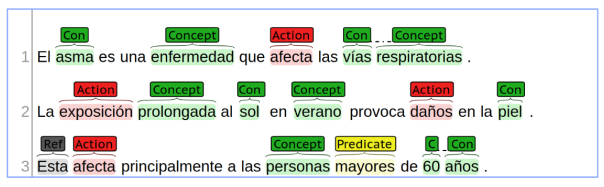
\includegraphics[width = 10cm]{Graphics/automaton.png}
	\caption{Función de decisión del autómata en la segunda etapa de la decodificación de la salida del modelo de extracción de entidades.}\label{fig:automaton}
\end{figure}

De acuerdo a evaluaciones efectuadas en las colecciones de entrenamiento y desarrollo, el proceso de decodificación de secuencias etiquetadas de manera correcta, extrae adecuadamente más del $98\%$ de las entidades presentes.


Luego de identificadas las entidades, para clasificar cada una de ellas de acuerdo a su tipo, se utiliza un sistema de votaci\'on, basado en la salida de la segunda capa CRF.
La misma asocia, para cada palabra en la oración de entrada, uno de los tipos de entidad, en este caso uno entre: \texttt{Concept}, \texttt{Action}, \texttt{Predicate} o \texttt{Reference}.
Cada palabra produce para cada entidad a la que pertenece, un voto de acuerdo al tipo que le fue asociado.
Luego, cada entidad se clasifica de según el tipo que mayor cantidad de votos que haya obtenido. Si está equilibrada la votación se asume \texttt{Concepto}, por ser la más frecuente por amplio margen en las colecciones estudiadas.



















